% =====================================================================
%  BÁO CÁO — Tấn công CSRF trên Elgg bằng Fetch API (Tiếng Việt)
%  Biên dịch: xelatex report_vi.tex  (chạy 2–3 lần để cập nhật mục lục)
% =====================================================================
\documentclass[11pt,a4paper]{article}

\usepackage{fontspec}
\setmainfont{TeX Gyre Termes}
\setsansfont{TeX Gyre Heros}
\setmonofont{Noto Sans Mono}[Scale=0.86]

\usepackage[vietnamese]{babel}

\usepackage[a4paper,margin=2.4cm,headheight=15pt]{geometry}
% =====================================================================
%  sty_common.tex — Shared visual style for the CSRF report (VI / EN)
%  Engine: XeLaTeX. Input AFTER \documentclass, fontspec fonts and babel.
% =====================================================================

% ---------- Colours (tie-in with the exploit page palette) -----------
\usepackage{xcolor}
\definecolor{navy}{HTML}{1E3C72}
\definecolor{brandblue}{HTML}{2A5298}
\definecolor{accent}{HTML}{2563EB}
\definecolor{danger}{HTML}{DC2626}
\definecolor{success}{HTML}{15803D}
\definecolor{amber}{HTML}{B45309}
\definecolor{ink}{HTML}{0F172A}
\definecolor{slate}{HTML}{475569}
\definecolor{mist}{HTML}{F1F5F9}
\definecolor{line}{HTML}{CBD5E1}
\definecolor{codebg}{HTML}{0F172A}
\definecolor{codefg}{HTML}{E2E8F0}
\definecolor{codekey}{HTML}{38BDF8}
\definecolor{codestr}{HTML}{86EFAC}
\definecolor{codecom}{HTML}{94A3B8}

% ---------- Graphics / diagrams --------------------------------------
\usepackage{graphicx}
\usepackage{tikz}
\usetikzlibrary{arrows.meta,positioning,calc,shadows.blur,backgrounds,fit}

% ---------- Tables ---------------------------------------------------
\usepackage{booktabs}
\usepackage{array}
\usepackage{tabularx}
\usepackage{colortbl}
\newcolumntype{Y}{>{\raggedright\arraybackslash}X}
\newcolumntype{C}{>{\centering\arraybackslash}X}

% ---------- Callout boxes --------------------------------------------
\usepackage[most]{tcolorbox}

\newtcolorbox{infobox}[1][]{
  enhanced, breakable, colback=mist, colframe=accent,
  boxrule=0pt, leftrule=3pt, arc=2pt, left=10pt, right=10pt,
  top=7pt, bottom=7pt, fonttitle=\bfseries\color{navy},
  coltitle=navy, title={#1}}

\newtcolorbox{warnbox}[1][]{
  enhanced, breakable, colback=danger!6, colframe=danger,
  boxrule=0pt, leftrule=3pt, arc=2pt, left=10pt, right=10pt,
  top=7pt, bottom=7pt, fonttitle=\bfseries, coltitle=danger, title={#1}}

\newtcolorbox{okbox}[1][]{
  enhanced, breakable, colback=success!6, colframe=success,
  boxrule=0pt, leftrule=3pt, arc=2pt, left=10pt, right=10pt,
  top=7pt, bottom=7pt, fonttitle=\bfseries, coltitle=success, title={#1}}

% ---------- Source-code listings (JS / Python / HTTP / bash) ---------
\usepackage{listings}
\lstset{
  basicstyle=\footnotesize\ttfamily\color{codefg},
  backgroundcolor=\color{codebg},
  keywordstyle=\color{codekey}\bfseries,
  stringstyle=\color{codestr},
  commentstyle=\color{codecom}\itshape,
  numberstyle=\tiny\color{codecom},
  frame=single, framerule=0pt, rulecolor=\color{codebg},
  numbers=left, numbersep=8pt, tabsize=2,
  showstringspaces=false, breaklines=true, breakatwhitespace=false,
  columns=fullflexible, keepspaces=true,
  xleftmargin=14pt, xrightmargin=6pt, aboveskip=10pt, belowskip=6pt,
  % Mono font (Noto Sans Mono) has full Vietnamese coverage -> no literate hacks.
  extendedchars=true, inputencoding=utf8,
}
% JavaScript dialect
\lstdefinelanguage{JavaScript}{
  keywords={const,let,var,function,async,await,return,try,catch,new,if,else,
            for,while,of,in,typeof,this,null,true,false,window,document},
  morekeywords=[2]{fetch,URLSearchParams,FormData,append,addEventListener},
  keywordstyle=[2]\color{codestr}\bfseries,
  sensitive=true,
  morecomment=[l]{//}, morecomment=[s]{/*}{*/},
  morestring=[b]', morestring=[b]", morestring=[b]`,
}
\lstdefinestyle{http}{
  language={}, morekeywords={POST,GET,HTTP,Host,Cookie,Content-Type,User-Agent,Accept,Connection},
}

% ---------- Icons via dingbats (no fontawesome dependency) -----------
\usepackage{pifont}
\newcommand{\yes}{\textcolor{success}{\ding{52}}}
\newcommand{\no}{\textcolor{danger}{\ding{56}}}
\newcommand{\step}[1]{\textcolor{white}{\colorbox{accent}{\footnotesize\bfseries~#1~}}}

% ---------- Misc -----------------------------------------------------
\usepackage{enumitem}
\setlist{leftmargin=1.4em,itemsep=2pt,topsep=3pt}
\usepackage{microtype}


\usepackage{fancyhdr}
\usepackage{titlesec}
\usepackage{lastpage}
\usepackage{hyperref}
\hypersetup{colorlinks=true,linkcolor=accent,urlcolor=accent,citecolor=accent,
  pdftitle={Tan cong CSRF tren Elgg bang Fetch API},
  pdfauthor={Nhom 6 - An toan may tinh}}

% ---- Section styling ----
\titleformat{\section}{\sffamily\Large\bfseries\color{navy}}{\thesection.}{0.6em}{}[{\color{line}\titlerule[1pt]}]
\titleformat{\subsection}{\sffamily\large\bfseries\color{brandblue}}{\thesubsection}{0.6em}{}
\titleformat{\subsubsection}{\sffamily\normalsize\bfseries\color{ink}}{\thesubsubsection}{0.6em}{}
\titlespacing*{\section}{0pt}{16pt}{8pt}

% ---- Header / footer ----
\pagestyle{fancy}
\fancyhf{}
\fancyhead[L]{\footnotesize\sffamily\color{slate}CSRF trên Elgg · Fetch API}
\fancyhead[R]{\footnotesize\sffamily\color{slate}An toàn máy tính — Nhóm 6}
\fancyfoot[C]{\footnotesize\sffamily\color{slate}Trang \thepage{} / \pageref{LastPage}}
\renewcommand{\headrulewidth}{0.4pt}
\renewcommand{\headrule}{\hbox to\headwidth{\color{line}\leaders\hrule height \headrulewidth\hfill}}

% =====================================================================
%  diagram_flow.tex — CSRF attack sequence diagram (\csrfflowdiagram)
%  Labels default to Vietnamese; an English document may \renewcommand
%  them BEFORE % =====================================================================
%  diagram_flow.tex — CSRF attack sequence diagram (\csrfflowdiagram)
%  Labels default to Vietnamese; an English document may \renewcommand
%  them BEFORE % =====================================================================
%  diagram_flow.tex — CSRF attack sequence diagram (\csrfflowdiagram)
%  Labels default to Vietnamese; an English document may \renewcommand
%  them BEFORE \input{diagram_flow}.
% =====================================================================
\providecommand{\lblVictim}{Alice (nạn nhân) + Trình duyệt}
\providecommand{\lblAttacker}{Attacker\\\texttt{attacker32.com}}
\providecommand{\lblElgg}{Elgg\\\texttt{seed-server.com}}
\providecommand{\lblSa}{1. Đăng nhập hợp lệ}
\providecommand{\lblSb}{2. Set-Cookie \texttt{Elgg=...}}
\providecommand{\lblSc}{3. Vô tình mở trang độc hại}
\providecommand{\lblSd}{4. Trả \texttt{index.html} (Fetch script)}
\providecommand{\lblNe}{5. Script tự chạy (\texttt{DOMContentLoaded})}
\providecommand{\lblSf}{6. Fetch POST + cookie (\texttt{credentials:'include'})}
\providecommand{\lblNg}{7. Cookie hợp lệ $\Rightarrow$ cập nhật About me}
\providecommand{\lblSh}{8. Phản hồi 302 (opaque)}
\providecommand{\lblSi}{9. Xem lại hồ sơ $\to$ đã bị đổi}

\newcommand{\csrfflowdiagram}{%
\begin{tikzpicture}[
   >={Stealth[length=2.4mm]}, font=\sffamily\scriptsize,
   head/.style={draw=navy,fill=navy,text=white,rounded corners=3pt,
                align=center,minimum height=0.85cm,minimum width=3.2cm,
                font=\sffamily\scriptsize\bfseries},
   life/.style={line,dashed,line width=0.7pt},
   msg/.style={->,accent,line width=0.9pt},
   ret/.style={->,slate,line width=0.7pt,dashed},
   note/.style={draw=amber,fill=amber!12,rounded corners=2pt,align=center,
                inner sep=3pt,font=\sffamily\scriptsize,text=amber!60!black}]

  \def\ax{0} \def\bx{5.4} \def\cx{10.8}
  \def\ytop{0} \def\ybot{-9.3}

  % lifeline heads
  \node[head] (A) at (\ax,\ytop) {\lblVictim};
  \node[head] (B) at (\bx,\ytop) {\lblAttacker};
  \node[head] (C) at (\cx,\ytop) {\lblElgg};

  % lifelines
  \draw[life] (\ax,-0.55) -- (\ax,\ybot);
  \draw[life] (\bx,-0.55) -- (\bx,\ybot);
  \draw[life] (\cx,-0.55) -- (\cx,\ybot);

  % messages
  \draw[msg] (\ax,-1.2) -- node[above]{\lblSa} (\cx,-1.2);
  \draw[ret] (\cx,-2.0) -- node[above]{\lblSb} (\ax,-2.0);
  \draw[msg] (\ax,-2.9) -- node[above]{\lblSc} (\bx,-2.9);
  \draw[ret] (\bx,-3.7) -- node[above]{\lblSd} (\ax,-3.7);

  \node[note,anchor=north west] at (\ax-1.7,-4.35) {\lblNe};

  \draw[msg,danger] (\ax,-5.6) -- node[above,text=danger]{\lblSf} (\cx,-5.6);

  \node[note,anchor=north] at (\cx,-6.2) {\lblNg};

  \draw[ret] (\cx,-7.4) -- node[above]{\lblSh} (\ax,-7.4);
  \draw[msg,success] (\ax,-8.4) -- node[above,text=success]{\lblSi} (\cx,-8.4);
\end{tikzpicture}%
}
.
% =====================================================================
\providecommand{\lblVictim}{Alice (nạn nhân) + Trình duyệt}
\providecommand{\lblAttacker}{Attacker\\\texttt{attacker32.com}}
\providecommand{\lblElgg}{Elgg\\\texttt{seed-server.com}}
\providecommand{\lblSa}{1. Đăng nhập hợp lệ}
\providecommand{\lblSb}{2. Set-Cookie \texttt{Elgg=...}}
\providecommand{\lblSc}{3. Vô tình mở trang độc hại}
\providecommand{\lblSd}{4. Trả \texttt{index.html} (Fetch script)}
\providecommand{\lblNe}{5. Script tự chạy (\texttt{DOMContentLoaded})}
\providecommand{\lblSf}{6. Fetch POST + cookie (\texttt{credentials:'include'})}
\providecommand{\lblNg}{7. Cookie hợp lệ $\Rightarrow$ cập nhật About me}
\providecommand{\lblSh}{8. Phản hồi 302 (opaque)}
\providecommand{\lblSi}{9. Xem lại hồ sơ $\to$ đã bị đổi}

\newcommand{\csrfflowdiagram}{%
\begin{tikzpicture}[
   >={Stealth[length=2.4mm]}, font=\sffamily\scriptsize,
   head/.style={draw=navy,fill=navy,text=white,rounded corners=3pt,
                align=center,minimum height=0.85cm,minimum width=3.2cm,
                font=\sffamily\scriptsize\bfseries},
   life/.style={line,dashed,line width=0.7pt},
   msg/.style={->,accent,line width=0.9pt},
   ret/.style={->,slate,line width=0.7pt,dashed},
   note/.style={draw=amber,fill=amber!12,rounded corners=2pt,align=center,
                inner sep=3pt,font=\sffamily\scriptsize,text=amber!60!black}]

  \def\ax{0} \def\bx{5.4} \def\cx{10.8}
  \def\ytop{0} \def\ybot{-9.3}

  % lifeline heads
  \node[head] (A) at (\ax,\ytop) {\lblVictim};
  \node[head] (B) at (\bx,\ytop) {\lblAttacker};
  \node[head] (C) at (\cx,\ytop) {\lblElgg};

  % lifelines
  \draw[life] (\ax,-0.55) -- (\ax,\ybot);
  \draw[life] (\bx,-0.55) -- (\bx,\ybot);
  \draw[life] (\cx,-0.55) -- (\cx,\ybot);

  % messages
  \draw[msg] (\ax,-1.2) -- node[above]{\lblSa} (\cx,-1.2);
  \draw[ret] (\cx,-2.0) -- node[above]{\lblSb} (\ax,-2.0);
  \draw[msg] (\ax,-2.9) -- node[above]{\lblSc} (\bx,-2.9);
  \draw[ret] (\bx,-3.7) -- node[above]{\lblSd} (\ax,-3.7);

  \node[note,anchor=north west] at (\ax-1.7,-4.35) {\lblNe};

  \draw[msg,danger] (\ax,-5.6) -- node[above,text=danger]{\lblSf} (\cx,-5.6);

  \node[note,anchor=north] at (\cx,-6.2) {\lblNg};

  \draw[ret] (\cx,-7.4) -- node[above]{\lblSh} (\ax,-7.4);
  \draw[msg,success] (\ax,-8.4) -- node[above,text=success]{\lblSi} (\cx,-8.4);
\end{tikzpicture}%
}
.
% =====================================================================
\providecommand{\lblVictim}{Alice (nạn nhân) + Trình duyệt}
\providecommand{\lblAttacker}{Attacker\\\texttt{attacker32.com}}
\providecommand{\lblElgg}{Elgg\\\texttt{seed-server.com}}
\providecommand{\lblSa}{1. Đăng nhập hợp lệ}
\providecommand{\lblSb}{2. Set-Cookie \texttt{Elgg=...}}
\providecommand{\lblSc}{3. Vô tình mở trang độc hại}
\providecommand{\lblSd}{4. Trả \texttt{index.html} (Fetch script)}
\providecommand{\lblNe}{5. Script tự chạy (\texttt{DOMContentLoaded})}
\providecommand{\lblSf}{6. Fetch POST + cookie (\texttt{credentials:'include'})}
\providecommand{\lblNg}{7. Cookie hợp lệ $\Rightarrow$ cập nhật About me}
\providecommand{\lblSh}{8. Phản hồi 302 (opaque)}
\providecommand{\lblSi}{9. Xem lại hồ sơ $\to$ đã bị đổi}

\newcommand{\csrfflowdiagram}{%
\begin{tikzpicture}[
   >={Stealth[length=2.4mm]}, font=\sffamily\scriptsize,
   head/.style={draw=navy,fill=navy,text=white,rounded corners=3pt,
                align=center,minimum height=0.85cm,minimum width=3.2cm,
                font=\sffamily\scriptsize\bfseries},
   life/.style={line,dashed,line width=0.7pt},
   msg/.style={->,accent,line width=0.9pt},
   ret/.style={->,slate,line width=0.7pt,dashed},
   note/.style={draw=amber,fill=amber!12,rounded corners=2pt,align=center,
                inner sep=3pt,font=\sffamily\scriptsize,text=amber!60!black}]

  \def\ax{0} \def\bx{5.4} \def\cx{10.8}
  \def\ytop{0} \def\ybot{-9.3}

  % lifeline heads
  \node[head] (A) at (\ax,\ytop) {\lblVictim};
  \node[head] (B) at (\bx,\ytop) {\lblAttacker};
  \node[head] (C) at (\cx,\ytop) {\lblElgg};

  % lifelines
  \draw[life] (\ax,-0.55) -- (\ax,\ybot);
  \draw[life] (\bx,-0.55) -- (\bx,\ybot);
  \draw[life] (\cx,-0.55) -- (\cx,\ybot);

  % messages
  \draw[msg] (\ax,-1.2) -- node[above]{\lblSa} (\cx,-1.2);
  \draw[ret] (\cx,-2.0) -- node[above]{\lblSb} (\ax,-2.0);
  \draw[msg] (\ax,-2.9) -- node[above]{\lblSc} (\bx,-2.9);
  \draw[ret] (\bx,-3.7) -- node[above]{\lblSd} (\ax,-3.7);

  \node[note,anchor=north west] at (\ax-1.7,-4.35) {\lblNe};

  \draw[msg,danger] (\ax,-5.6) -- node[above,text=danger]{\lblSf} (\cx,-5.6);

  \node[note,anchor=north] at (\cx,-6.2) {\lblNg};

  \draw[ret] (\cx,-7.4) -- node[above]{\lblSh} (\ax,-7.4);
  \draw[msg,success] (\ax,-8.4) -- node[above,text=success]{\lblSi} (\cx,-8.4);
\end{tikzpicture}%
}


\begin{document}
\selectlanguage{vietnamese}

% =====================================================================
%  TRANG BÌA
% =====================================================================
\begin{titlepage}
\begin{tikzpicture}[remember picture,overlay]
  \fill[navy] (current page.north west) rectangle ([yshift=-5.2cm]current page.north east);
  \fill[brandblue] ([yshift=-5.2cm]current page.north west) rectangle ([yshift=-5.7cm]current page.north east);
  \node[anchor=north west,text=white,font=\sffamily\small] at ([xshift=2.4cm,yshift=-1.1cm]current page.north west)
     {ĐẠI HỌC QUỐC GIA HÀ NỘI — TRƯỜNG ĐẠI HỌC KHOA HỌC TỰ NHIÊN};
  \node[anchor=north west,text=white,font=\sffamily\small] at ([xshift=2.4cm,yshift=-1.7cm]current page.north west)
     {Học phần: An toàn máy tính};
  \node[anchor=north west,text=white,font=\sffamily\bfseries\LARGE,text width=16cm] at ([xshift=2.4cm,yshift=-3.0cm]current page.north west)
     {Báo cáo Thực hành};
  \node[anchor=north west,text=mist,font=\sffamily\large,text width=16cm] at ([xshift=2.4cm,yshift=-4.2cm]current page.north west)
     {Tấn công Cross-Site Request Forgery (CSRF)};
\end{tikzpicture}

\vspace*{6.2cm}
{\sffamily
\begin{flushleft}
{\color{slate}\large ĐỀ TÀI}\\[4pt]
{\color{navy}\bfseries\Huge Tấn công CSRF trên nền tảng\\[6pt] mạng xã hội Elgg bằng Fetch API}\\[14pt]
{\color{ink}\large Thay thế XMLHttpRequest / Form submit bằng \texttt{fetch()} + \texttt{URLSearchParams} / \texttt{FormData}}
\end{flushleft}}

\vfill
{\sffamily\normalsize
\begin{tcolorbox}[colback=mist,colframe=line,boxrule=0.6pt,arc=3pt]
\begin{tabularx}{\linewidth}{@{}l Y@{}}
\textbf{Nhóm thực hiện} & Nhóm 6 (03 thành viên)\\[3pt]
\textbf{Nguyễn Trung Thành} & MSV 23001935 \quad — Lý thuyết, phân tích HTTP, phòng chống\\[3pt]
\textbf{Nguyễn Công Trí} & MSV 23001939 \quad — Elgg, Docker, Fetch API, kiểm thử\\[3pt]
\textbf{Nguyễn Minh Thao} & MSV 23001936 \quad — Bằng chứng, PowerPoint, video\\[3pt]
\textbf{Giảng viên} & \underline{\hspace{6cm}}\\[3pt]
\textbf{Ngày báo cáo} & \today\\
\end{tabularx}
\end{tcolorbox}}

\begin{center}\footnotesize\color{slate}
\textbf{Lưu ý đạo đức:} Toàn bộ nội dung chỉ phục vụ học tập trong môi trường lab cục bộ (Docker) do nhóm sở hữu — không nhằm tác động tới bất kỳ cá nhân/tổ chức nào.
\end{center}
\end{titlepage}

% =====================================================================
%  TÓM TẮT + MỤC LỤC
% =====================================================================
\begin{abstract}
\noindent Báo cáo trình bày quá trình nghiên cứu và thực nghiệm tấn công \textbf{Cross-Site Request Forgery (CSRF)} trên ứng dụng mạng xã hội mã nguồn mở \textbf{Elgg}. Điểm cải tiến so với bài lab gốc là thay thế hoàn toàn \texttt{XMLHttpRequest} và cơ chế \texttt{form submit} bằng \textbf{Fetch API} hiện đại kết hợp \texttt{URLSearchParams} hoặc \texttt{FormData}. Mục tiêu khai thác là thay đổi trường \emph{About me} trong hồ sơ nạn nhân thành chuỗi \texttt{CSRF attack by <MSV>}.

Khác với nhiều báo cáo chỉ dừng ở mô tả, nhóm đã \textbf{dựng và chạy thật} một lab Docker cục bộ (Elgg \textbf{3.3.3}, cô lập loopback), ghi lại \textbf{ảnh chụp màn hình thực tế} từ trình duyệt Chrome và kiểm chứng kết quả ở cả tầng giao diện lẫn tầng HTTP. Báo cáo phân tích gói tin HTTP, giải thích các cơ chế cốt lõi (\texttt{credentials: 'include'}, Simple Request, \texttt{mode: 'no-cors'}), minh hoạ sơ đồ luồng tấn công, trình bày một \textbf{phát hiện kỹ thuật} về cách Elgg lưu trường hồ sơ (annotation so với metadata), và — quan trọng nhất — \textbf{chứng minh bằng thực nghiệm} hiệu quả của hai lớp phòng thủ độc lập: \emph{anti-CSRF token} và \emph{cookie SameSite}. Cuối báo cáo tổng hợp lời giải 15 câu hỏi lý thuyết, quy trình tái hiện và bản khai báo mức độ sử dụng AI.
\end{abstract}

{\hypersetup{linkcolor=ink}\tableofcontents}
\newpage

% =====================================================================
\section{Giới thiệu và mục tiêu}
\subsection{Bối cảnh}
CSRF là lỗ hổng ở tầng logic ứng dụng web, khai thác cơ chế \emph{tin cậy ngầm định} của trình duyệt: khi gửi một yêu cầu đến một tên miền, trình duyệt tự động đính kèm toàn bộ cookie thuộc tên miền đó — bao gồm cả cookie phiên xác thực. Kẻ tấn công lợi dụng điều này để khiến trình duyệt của nạn nhân (đang đăng nhập) gửi đi một yêu cầu thay đổi trạng thái mà nạn nhân không chủ ý. Điểm nguy hiểm là kẻ tấn công \emph{không cần biết mật khẩu}, cũng không cần đánh cắp cookie: nó chỉ cần \emph{mượn} phiên đăng nhập sẵn có của nạn nhân trong khoảnh khắc nạn nhân ghé thăm một trang web độc hại.

\subsection{Mục tiêu đề tài}
\begin{itemize}
  \item \textbf{Hệ thống mục tiêu:} ứng dụng Elgg chạy trong container Docker; tài khoản nạn nhân giả lập là \emph{Alice}.
  \item \textbf{Hành vi khai thác:} từ một trang web của kẻ tấn công (khác origin), giả mạo một HTTP POST tới endpoint \texttt{/action/profile/edit} để đổi trường \emph{About me} của nạn nhân thành \texttt{CSRF attack by 23001939}.
  \item \textbf{Ràng buộc kỹ thuật bắt buộc:}
  \begin{enumerate}
    \item \no{} Không dùng \texttt{XMLHttpRequest}.
    \item \no{} Không dùng \texttt{<form>} tự submit (gây chuyển hướng, lộ dấu vết).
    \item \yes{} Bắt buộc dùng \textbf{Fetch API} + \texttt{URLSearchParams} hoặc \texttt{FormData}.
  \end{enumerate}
  \item \textbf{Yêu cầu minh chứng:} đổi được About me đồng thời \emph{chứng minh} được vì sao tấn công thành công khi thiếu phòng vệ và thất bại khi bật phòng vệ.
\end{itemize}

\begin{warnbox}[Phạm vi \& đạo đức]
Mọi thao tác chỉ thực hiện trong môi trường lab cục bộ do nhóm sở hữu, cô lập trên \texttt{localhost}. Việc áp dụng các kỹ thuật này lên hệ thống không được cấp phép là vi phạm pháp luật và quy chế học thuật. Mục đích duy nhất là \emph{học tấn công để biết cách phòng thủ}.
\end{warnbox}

% =====================================================================
\section{Cơ sở lý thuyết CSRF}
\subsection{Ba điều kiện của một cuộc tấn công}
\begin{enumerate}
  \item Nạn nhân có \textbf{phiên đăng nhập còn hiệu lực} (session cookie) với ứng dụng mục tiêu.
  \item Hành động mục tiêu \textbf{thay đổi trạng thái} (đổi hồ sơ, chuyển tiền, kết bạn\ldots) và có tham số \textbf{dự đoán được}.
  \item Ứng dụng \textbf{thiếu cơ chế phòng vệ} (không SameSite Strict/Lax, không anti-CSRF token, không kiểm tra \texttt{Origin}).
\end{enumerate}
Nếu thiếu bất kỳ điều kiện nào, cuộc tấn công sẽ không thành công — đây cũng chính là cơ sở để thiết kế biện pháp phòng thủ (Mục~\ref{sec:defense}).

\subsection{Cơ chế cookie và sự tin cậy ngầm định}
Khi Alice đăng nhập, Elgg phát một cookie phiên (ví dụ \texttt{Elgg=p8nm1rqhk8\ldots}) và lưu trong trình duyệt, gắn với host của Elgg. \textbf{Quy tắc máy móc} của trình duyệt là: \emph{mọi} request gửi \emph{tới} host đó sẽ \emph{tự động} kèm cookie, bất kể request được khởi tạo từ trang nào. Trình duyệt quyết định đính cookie dựa trên \emph{đích đến} của request, chứ không dựa trên \emph{nguồn gốc} của trang phát ra nó. Chính sự "vô tư" này tạo ra lỗ hổng CSRF.

\subsection{Same-Origin, Same-Site và cross-site}
\begin{center}\small
\begin{tabularx}{\linewidth}{@{}l Y Y@{}}
\toprule
\textbf{Khái niệm} & \textbf{Định nghĩa} & \textbf{Ví dụ trong lab}\\
\midrule
Same-origin & Trùng cả \emph{scheme + host + port} & \texttt{elgg.csrf.localhost:8080} với chính nó\\
Same-site & Trùng \emph{site} (eTLD+1), có thể khác subdomain/port & \texttt{attacker.csrf.localhost} \& \texttt{elgg.csrf.localhost} (cùng site \texttt{csrf.localhost})\\
Cross-site & Khác site (khác eTLD+1) & \texttt{127.0.0.1} với \texttt{elgg.csrf.localhost}\\
\bottomrule
\end{tabularx}
\end{center}
\noindent Sự phân biệt \emph{same-site} với \emph{cross-site} là mấu chốt để hiểu cookie \texttt{SameSite}: thuộc tính này chặn cookie trong request \emph{cross-site} nhưng vẫn cho phép trong request \emph{same-site}. Lab của nhóm cố ý bố trí hai trang attacker — một \emph{cùng-site} và một \emph{khác-site} — để tách bạch vai trò của SameSite (xem Mục~\ref{sec:result}).

\subsection{Khe hở ``gửi được nhưng không đọc được''}
Chính sách Same-Origin Policy (SOP) cấm JavaScript của trang này \emph{đọc} nội dung/response của trang khác origin — nhưng \textbf{không} cấm \emph{gửi} yêu cầu. Chính khe hở này là nền tảng của CSRF: kẻ tấn công không cần đọc kết quả, chỉ cần hành động thay đổi trạng thái được thực thi ở phía server. Đây cũng là lý do \texttt{mode: 'no-cors'} (response \emph{opaque}, JS không đọc được) vẫn đủ để tấn công thành công.

\subsection{Phân biệt CSRF với XSS}
Cần tránh nhầm lẫn: \textbf{XSS} chèn và chạy mã trong ngữ cảnh trang nạn nhân (đọc được cookie, token\ldots), còn \textbf{CSRF} \emph{không} đọc được gì của trang mục tiêu — nó chỉ \emph{lợi dụng} việc trình duyệt tự đính cookie. Vì vậy anti-CSRF token chống được CSRF (attacker không đọc được token) nhưng \emph{không} chống được XSS (mã XSS chạy trong trang nên đọc được token).

\subsection{Mô hình mối đe dọa (Threat Model)}
\begin{center}\small
\begin{tabularx}{\linewidth}{@{}l Y@{}}
\toprule
\textbf{Yếu tố} & \textbf{Mô tả trong lab}\\
\midrule
Tài sản cần bảo vệ & Tính toàn vẹn hồ sơ người dùng (trường About me)\\
Kẻ tấn công & Chủ trang web độc hại, \emph{không} có quyền truy cập máy chủ Elgg, \emph{không} biết mật khẩu Alice\\
Năng lực của attacker & Khiến trình duyệt Alice phát một request; \emph{không} đọc được response (SOP)\\
Điều kiện kích hoạt & Alice đang đăng nhập và ghé trang attacker\\
Mục tiêu attacker & Thực thi hành động đổi trạng thái thay Alice mà cô không chủ ý\\
\bottomrule
\end{tabularx}
\end{center}
\noindent Mô hình này cho thấy CSRF là lỗ hổng \emph{lạm quyền ngầm}: attacker mượn \emph{thẩm quyền} của phiên đăng nhập, chứ không trộm thông tin xác thực. Hệ quả: nguyên tắc thiết kế an toàn là \emph{không} dùng \texttt{GET} cho hành động đổi trạng thái, và luôn ràng buộc hành động với một bằng chứng ``người dùng thực sự chủ ý'' (token/Origin/SameSite).

% =====================================================================
\section{Hai mô hình môi trường thực nghiệm}
\subsection{Mô hình chuẩn SEED Labs}
Bài lab CSRF gốc của bộ SEED Labs dùng ba container với tên miền ảo ánh xạ qua \texttt{/etc/hosts}:
\begin{center}\small
\begin{tabularx}{\linewidth}{@{}l l Y@{}}
\toprule
\textbf{Dịch vụ} & \textbf{Địa chỉ} & \textbf{Vai trò}\\
\midrule
seed-server & \texttt{www.seed-server.com} (10.9.0.5) & Apache + ứng dụng Elgg (mục tiêu)\\
mysql       & 10.9.0.6 & Cơ sở dữ liệu người dùng Elgg\\
attacker32  & \texttt{www.attacker32.com} (10.9.0.7) & Máy chủ web của kẻ tấn công\\
\bottomrule
\end{tabularx}
\end{center}
\noindent Mô hình này là \emph{khung khái niệm} chuẩn để trình bày lý thuyết; tuy nhiên hai host đều là cùng-site (\texttt{*.com} khác nhau nên thực tế là cross-site) và phụ thuộc việc tắt token sẵn trong ảnh SEED.

\subsection{Lab Docker cục bộ của nhóm (đã chạy thật)}
Để kiểm soát chính xác điều kiện thí nghiệm và lấy bằng chứng thật, nhóm dựng một lab riêng, cô lập hoàn toàn trên loopback:
\begin{center}\small
\begin{tabularx}{\linewidth}{@{}l l Y@{}}
\toprule
\textbf{Thành phần} & \textbf{URL} & \textbf{Vai trò / điều kiện}\\
\midrule
Elgg (nạn nhân) & \texttt{elgg.csrf.localhost:8080} & Elgg \textbf{3.3.3}, cookie host-only, HTTP loopback\\
Attacker cùng-site & \texttt{attacker.csrf.localhost:8000} & Khác origin, \emph{cùng site} \texttt{csrf.localhost}\\
Attacker khác-site & \texttt{127.0.0.1:8000} & \emph{Khác site} so với Elgg\\
MySQL & (trong Docker network) & 8.0.37, không publish cổng ra ngoài\\
\bottomrule
\end{tabularx}
\end{center}
\begin{figure}[h]\centering
\begin{tikzpicture}[font=\sffamily\scriptsize,>={Stealth[length=2mm]},
  box/.style={rounded corners=3pt,draw,align=center,minimum height=1.05cm,minimum width=3.1cm},
  victim/.style={box,draw=navy,fill=navy!8,text=ink},
  elgg/.style={box,draw=success,fill=success!8},
  atk/.style={box,draw=danger,fill=danger!6},
  db/.style={box,draw=slate,fill=mist},
  lbl/.style={font=\sffamily\scriptsize\itshape,text=slate}]
  \node[victim] (chrome) {Chrome (Alice)\\\scriptsize cookie \texttt{Elgg=...}};
  \node[atk,above right=0.35cm and 2.6cm of chrome] (a1) {Attacker \textbf{cùng-site}\\\texttt{attacker.csrf.localhost:8000}};
  \node[atk,below right=0.35cm and 2.6cm of chrome] (a2) {Attacker \textbf{khác-site}\\\texttt{127.0.0.1:8000}};
  \node[elgg,right=6.2cm of chrome] (elgg) {Elgg 3.3.3\\\texttt{elgg.csrf.localhost:8080}};
  \node[db,below=0.5cm of elgg] (db) {MySQL 8.0.37\\\scriptsize (internal network)};
  \draw[->,danger] (a1.east) .. controls +(1.2,0) and +(-1.2,0.5) .. (elgg.west) node[midway,above,lbl,text=danger]{POST (same-site)};
  \draw[->,danger,dashed] (a2.east) .. controls +(1.2,0) and +(-1.2,-0.5) .. (elgg.west) node[midway,below,lbl,text=danger]{POST (cross-site)};
  \draw[->,navy] (chrome) -- (a1.west);
  \draw[->,navy] (chrome) -- (a2.west);
  \draw[<->,slate] (elgg) -- (db);
\end{tikzpicture}
\\[3pt]\footnotesize\color{slate}Kiến trúc lab: trình duyệt Alice, hai trang attacker (cùng-site / khác-site), Elgg và MySQL.
\end{figure}

\noindent Phiên bản ứng dụng được xác minh runtime bằng lệnh \texttt{labctl version}: Elgg \texttt{3.3.3}, digest ảnh \texttt{sha256:5d8a25b1\ldots708f7f5}. Lab có \textbf{hai chế độ} chuyển bằng công cụ \texttt{labctl}:
\begin{itemize}
  \item \texttt{protected} (mặc định): Elgg kiểm tra \texttt{\_\_elgg\_token}/\texttt{\_\_elgg\_ts} như bình thường $\Rightarrow$ tấn công \emph{phải thất bại}.
  \item \texttt{vulnerable}: tắt kiểm tra token \emph{chỉ cho} action \texttt{/action/profile/edit} $\Rightarrow$ minh họa hậu quả khi mất lớp phòng vệ.
\end{itemize}

\begin{infobox}[Vì sao có hai host attacker?]
Việc đặt một attacker \emph{cùng-site} và một \emph{khác-site} cho phép thay đổi \textbf{đúng một biến} mỗi lần: giữ nguyên chế độ \texttt{vulnerable} (token đã tắt) và chỉ đổi \emph{cùng-site $\leftrightarrow$ khác-site}. Nếu kết quả khác nhau, nguyên nhân \emph{chỉ có thể} là cookie \texttt{SameSite}. Đây là phương pháp kiểm soát biến để quy kết nguyên nhân một cách chặt chẽ.
\end{infobox}

\subsection{So sánh hai mô hình}
Mô hình SEED chuẩn dùng để giảng giải khái niệm và đối chiếu tài liệu; lab Docker cục bộ dùng để \emph{chạy thật, lấy bằng chứng và kiểm soát biến}. Hai mô hình bổ trợ nhau: khái niệm rút ra từ SEED được \emph{kiểm chứng} trên lab thật của nhóm. Các mục kết quả (Mục~\ref{sec:result}) và phòng thủ (Mục~\ref{sec:defense}) đều dựa trên lab Docker đã chạy.

% =====================================================================
\section{Phân tích HTTP request bằng DevTools}
Để giả mạo chính xác, trước tiên phải bắt một request hợp lệ. Đăng nhập Alice (\texttt{alice}/\texttt{seedalice}), vào \emph{Edit Profile}, mở \texttt{F12 → Network} (bật \emph{Preserve log}), sửa trường About me rồi bấm \textbf{Save}.

\begin{lstlisting}[style=http,caption={Request POST khi lưu hồ sơ (rút gọn, từ lab thật)}]
POST /action/profile/edit HTTP/1.1
Host: elgg.csrf.localhost:8080
Content-Type: application/x-www-form-urlencoded
Cookie: Elgg=p8nm1rqhk8igl0ivf1i5qkdl3m; ...

name=Alice&description=<p>...</p>&accesslevel[description]=2
&guid=56&__elgg_ts=1794550779&__elgg_token=RG40vT3Fxs...
\end{lstlisting}

\begin{center}\small
\begin{tabularx}{\linewidth}{@{}l Y l@{}}
\toprule
\textbf{Tham số} & \textbf{Ý nghĩa} & \textbf{Giá trị (lab)}\\
\midrule
\texttt{guid} & ID định danh nạn nhân (Alice) & \texttt{56}\\
\texttt{name} & Tên hiển thị & \texttt{Alice}\\
\texttt{description} & \textbf{Nội dung About me} & \texttt{CSRF attack by 23001939}\\
\texttt{accesslevel[description]} & Quyền xem (2 = Public) & \texttt{2}\\
\texttt{\_\_elgg\_token / \_\_elgg\_ts} & Anti-CSRF token + timestamp & \emph{(bí mật — KHÔNG đưa sang attacker)}\\
\bottomrule
\end{tabularx}
\end{center}

\subsection{Quy trình bắt request bằng tab Network}
\begin{enumerate}
  \item Mở \texttt{F12 → Network}, bật \emph{Preserve log} để không mất request khi trang chuyển hướng.
  \item Thực hiện một thao tác hợp lệ (Save hồ sơ); tìm request \texttt{POST} tới \texttt{/action/profile/edit}.
  \item Xem tab \emph{Payload}/\emph{Request} để đọc các trường và tab \emph{Headers} để xác nhận \texttt{Content-Type}, \texttt{Cookie}.
  \item Ghi lại \emph{endpoint} và \emph{các trường công khai}; xác nhận sự tồn tại của \texttt{\_\_elgg\_token} nhưng \textbf{không} sao chép giá trị của nó.
\end{enumerate}

\begin{warnbox}[Nguyên tắc vàng khi bắt request]
Chỉ sao chép các \emph{trường công khai} (\texttt{guid}, \texttt{name}, \texttt{description}, \texttt{accesslevel}) sang trang attacker. \textbf{Tuyệt đối không} nhập \texttt{\_\_elgg\_token}, \texttt{\_\_elgg\_ts}, cookie hay mật khẩu vào attacker — làm vậy là tự ``đưa chìa khóa cho mình'', phá vỡ ý nghĩa của thí nghiệm. Công cụ attacker của nhóm chủ động \emph{từ chối} mọi trường chứa \texttt{token}/\texttt{cookie}/\texttt{password}.
\end{warnbox}

% =====================================================================
\section{Kỹ thuật khai thác bằng Fetch API}
\subsection{So sánh ba phương pháp}
\begin{center}\small
\begin{tabularx}{\linewidth}{@{}Y C C C@{}}
\toprule
\textbf{Tiêu chí} & \textbf{Form submit} & \textbf{XHR} & \textbf{Fetch API}\\
\midrule
Tàng hình (không chuyển trang) & \no & \yes & \yes\\
Cú pháp hiện đại (Promise/async) & \no & \no & \yes\\
Kiểm soát \texttt{mode}/\texttt{credentials} & hạn chế & có & \yes{} rõ ràng\\
Tuân thủ đề bài & \no{} cấm & \no{} cấm & \yes{} bắt buộc\\
\bottomrule
\end{tabularx}
\end{center}

\subsection{Hai cơ chế then chốt}
\begin{infobox}[\texttt{credentials: 'include'} — gửi cookie qua cross-origin]
Mặc định, \texttt{fetch()} cross-origin dùng \texttt{credentials: 'same-origin'} nên \emph{không} gửi cookie của Elgg. Phải đặt \texttt{credentials: 'include'} để trình duyệt tự đính kèm cookie phiên của nạn nhân — nếu thiếu, server coi là khách vãng lai và tấn công thất bại. Lưu ý: cờ này chỉ là \emph{lời đề nghị}; trình duyệt vẫn có quyền từ chối đính cookie nếu cookie mang thuộc tính \texttt{SameSite} và request là cross-site.
\end{infobox}

\begin{infobox}[Simple Request + \texttt{mode: 'no-cors'} — vượt Preflight]
\texttt{Content-Type} dạng \texttt{application/x-www-form-urlencoded} (URLSearchParams) hoặc \texttt{multipart/form-data} (FormData) đều thuộc nhóm \emph{CORS-safelisted} $\Rightarrow$ đây là \textbf{Simple Request}, không phát sinh Preflight \texttt{OPTIONS}. Dù SOP chặn JavaScript \emph{đọc} response (opaque), server Elgg \emph{vẫn} nhận cookie hợp lệ và ghi đè cơ sở dữ liệu thành công.
\end{infobox}

\subsection{Mã khai thác (biến thể URLSearchParams)}
\begin{lstlisting}[language=JavaScript,caption={Lõi tấn công bằng Fetch API + URLSearchParams}]
const payload = new URLSearchParams();
payload.append('name', 'Alice');
payload.append('description', 'CSRF attack by 23001939');
payload.append('accesslevel[description]', '2');   // 2 = Public
payload.append('guid', '56');                       // Alice's GUID

fetch('http://elgg.csrf.localhost:8080/action/profile/edit', {
  method: 'POST',
  mode: 'no-cors',          // Simple Request -> no Preflight OPTIONS
  credentials: 'include',   // REQUIRED: attach victim's session cookie
  body: payload             // URLSearchParams tu sinh Content-Type an toan
});
\end{lstlisting}

\subsection{Mã khai thác (biến thể FormData)}
\begin{lstlisting}[language=JavaScript,caption={Biến thể Fetch API + FormData}]
const payload = new FormData();
payload.append('name', 'Alice');
payload.append('description', 'CSRF attack by 23001939');
payload.append('accesslevel[description]', '2');
payload.append('guid', '56');

fetch('http://elgg.csrf.localhost:8080/action/profile/edit', {
  method: 'POST',
  mode: 'no-cors',
  credentials: 'include',
  body: payload            // KHONG dat Content-Type: trinh duyet tu sinh boundary
});
\end{lstlisting}

\begin{infobox}[URLSearchParams hay FormData?]
Cả hai đều tạo \emph{Simple Request} nên không phát sinh Preflight. \texttt{URLSearchParams} sinh \texttt{application/x-www-form-urlencoded} (gọn, hợp với form đơn giản); \texttt{FormData} sinh \texttt{multipart/form-data} với \texttt{boundary} (hợp khi có tệp đính kèm). Điểm mấu chốt chung: \textbf{không} tự đặt header \texttt{Content-Type} để trình duyệt giữ giá trị \emph{safelisted}. Nhóm cung cấp cả hai biến thể trong mã nguồn.
\end{infobox}

% =====================================================================
\section{Sơ đồ luồng tấn công}
\begin{center}
\scalebox{0.92}{\csrfflowdiagram}
\end{center}
\noindent Sơ đồ tuần tự: (1--2) Alice đăng nhập, nhận cookie. (3--5) Alice vô tình mở trang attacker, script Fetch tự chạy. (6) Fetch POST kèm cookie (nhờ \texttt{credentials:'include'}). (7) Nếu thiếu phòng vệ, Elgg cập nhật About me. (8--9) Response opaque; Alice tải lại hồ sơ thì thấy đã bị đổi.

% =====================================================================
\section{Kết quả thực nghiệm trên lab thật}\label{sec:result}
Nhóm chạy toàn bộ kịch bản trên trình duyệt Chrome thật (điều khiển qua automation) và đối chiếu từng bước. Phiên bản Elgg xác minh: \textbf{3.3.3}.

\subsection{Ma trận ca kiểm thử}
\begin{center}\small
\begin{tabularx}{\linewidth}{@{}l l c c Y c@{}}
\toprule
\textbf{Mã TC} & \textbf{Chế độ} & \textbf{Attacker} & \textbf{Same-site?} & \textbf{Kỳ vọng} & \textbf{KQ}\\
\midrule
TC-B01 & protected & — (UI Elgg) & — & Save hợp lệ; request có token & \yes\\
TC-B04 & protected & cùng-site & có & Bị chặn, About me giữ nguyên & \yes\\
TC-B03 & vulnerable & \texttt{127.0.0.1} & \textbf{không} & Bị chặn bởi SameSite & \yes\\
TC-B05/06 & vulnerable & cùng-site & có & \textbf{Thành công}, About me đổi & \yes\\
\bottomrule
\end{tabularx}
\end{center}
\noindent Chỉ đổi \emph{một} biến giữa TC-B03 và TC-B05/06 (khác-site $\leftrightarrow$ cùng-site). Kết quả trái ngược (chặn $\leftrightarrow$ thành công) chính là minh chứng cho vai trò của cookie \texttt{SameSite}.

\subsection{Bằng chứng hình ảnh}
\begin{figure}[h]\centering
\begin{minipage}[t]{0.48\linewidth}\centering
  \fbox{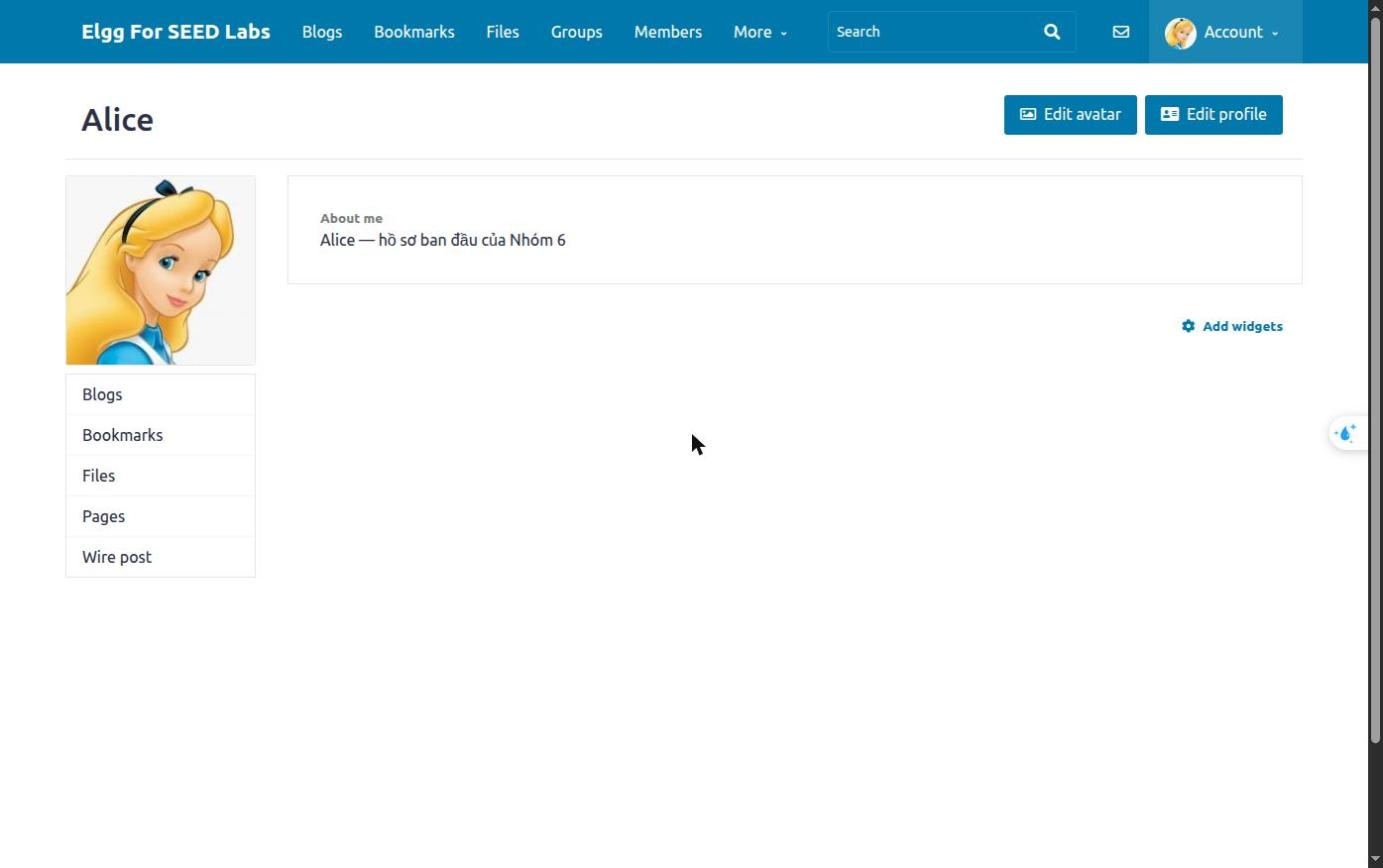
\includegraphics[width=\linewidth]{img/ev-before.jpg}}
  \\[3pt]\footnotesize\color{slate}(a) \textbf{Trước:} About me baseline của Alice.
\end{minipage}\hfill
\begin{minipage}[t]{0.48\linewidth}\centering
  \fbox{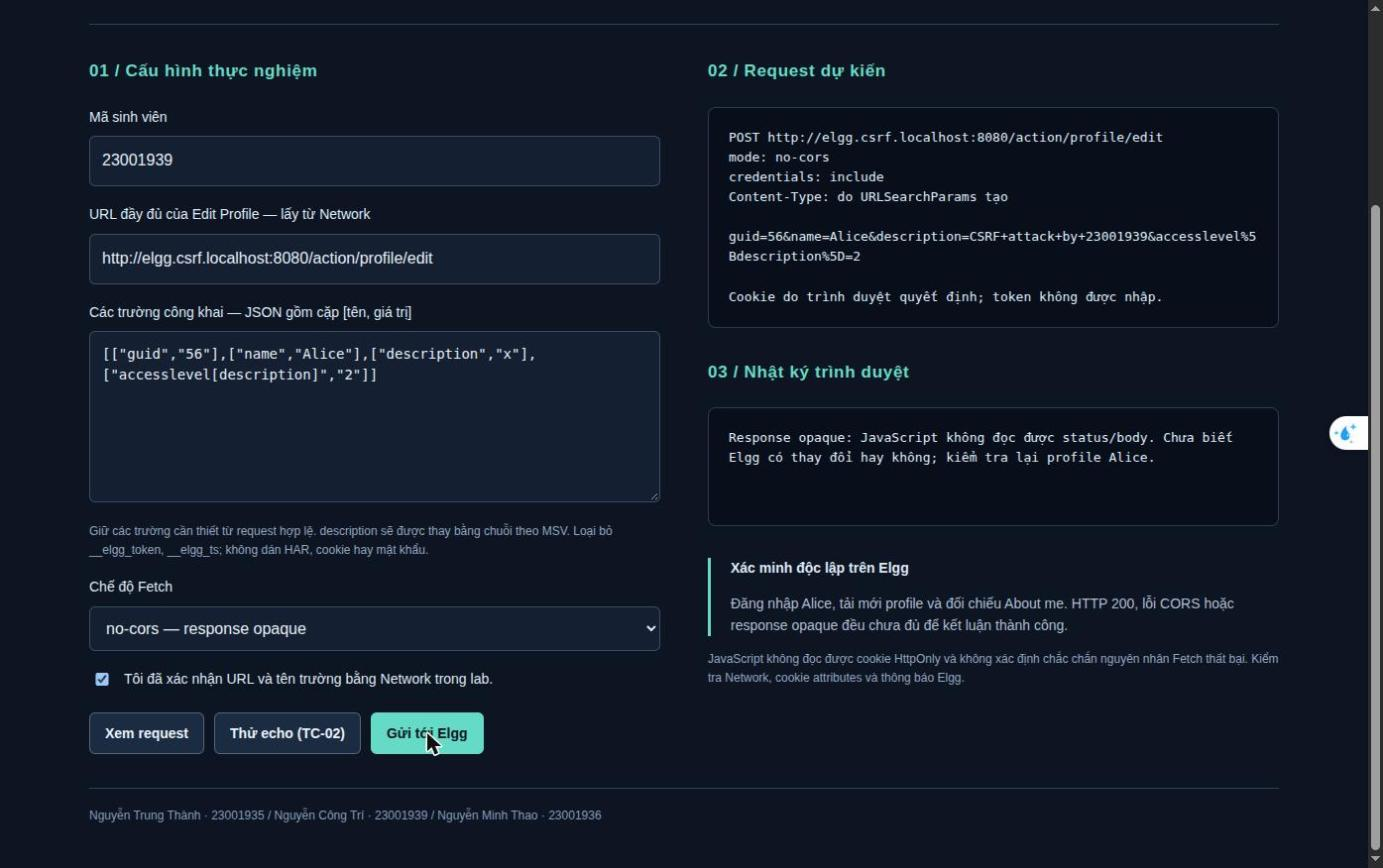
\includegraphics[width=\linewidth]{img/ev-attacker-payload.jpg}}
  \\[3pt]\footnotesize\color{slate}(b) Trang attacker: payload Fetch dự kiến, \emph{không} có token.
\end{minipage}
\end{figure}

\begin{figure}[h]\centering
\begin{minipage}[t]{0.48\linewidth}\centering
  \fbox{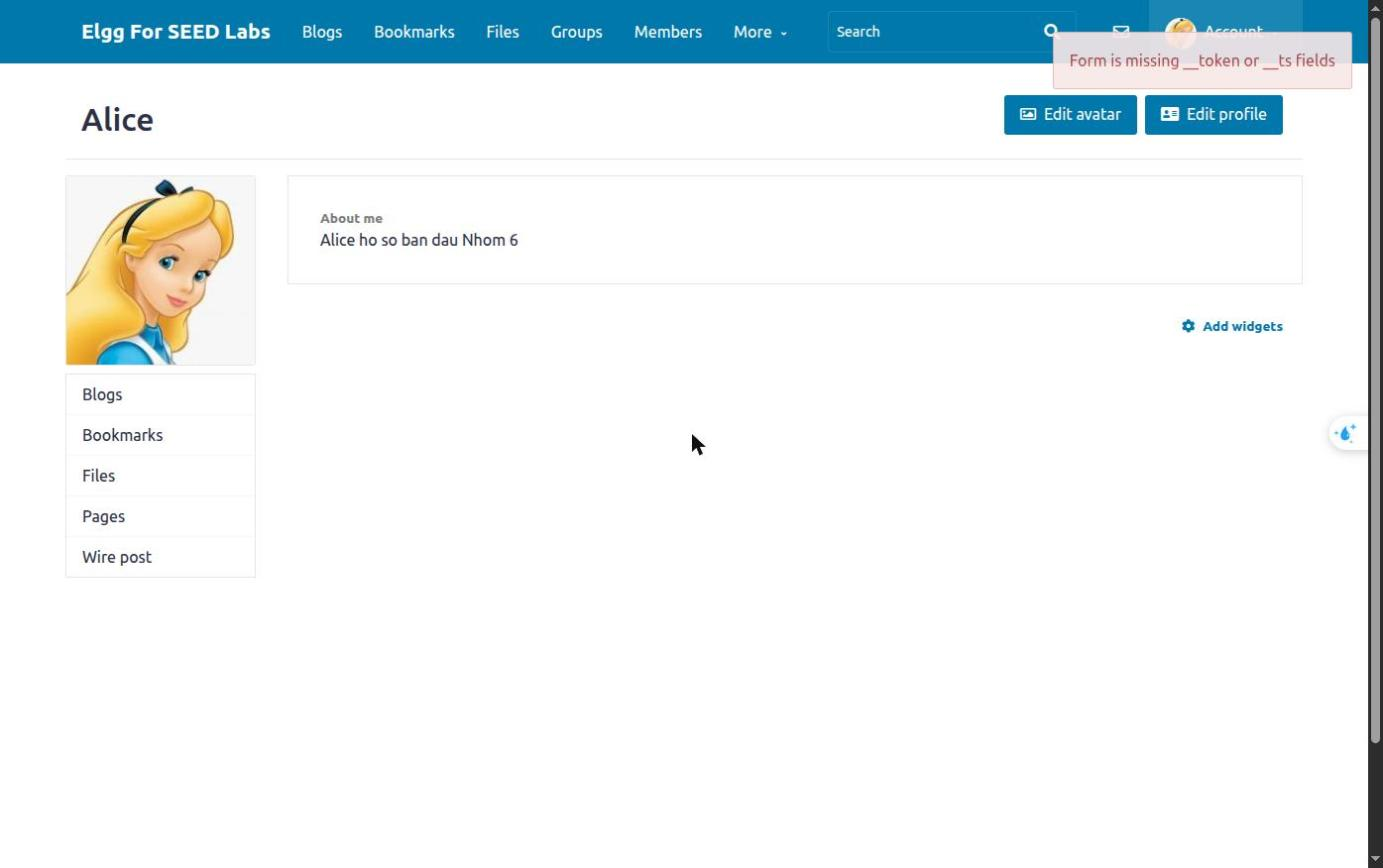
\includegraphics[width=\linewidth]{img/ev-protected-blocked.jpg}}
  \\[3pt]\footnotesize\color{slate}(c) \textbf{TC-B04 (protected):} Elgg báo \emph{``Form is missing \_\_token or \_\_ts fields''}; About me không đổi.
\end{minipage}\hfill
\begin{minipage}[t]{0.48\linewidth}\centering
  \fbox{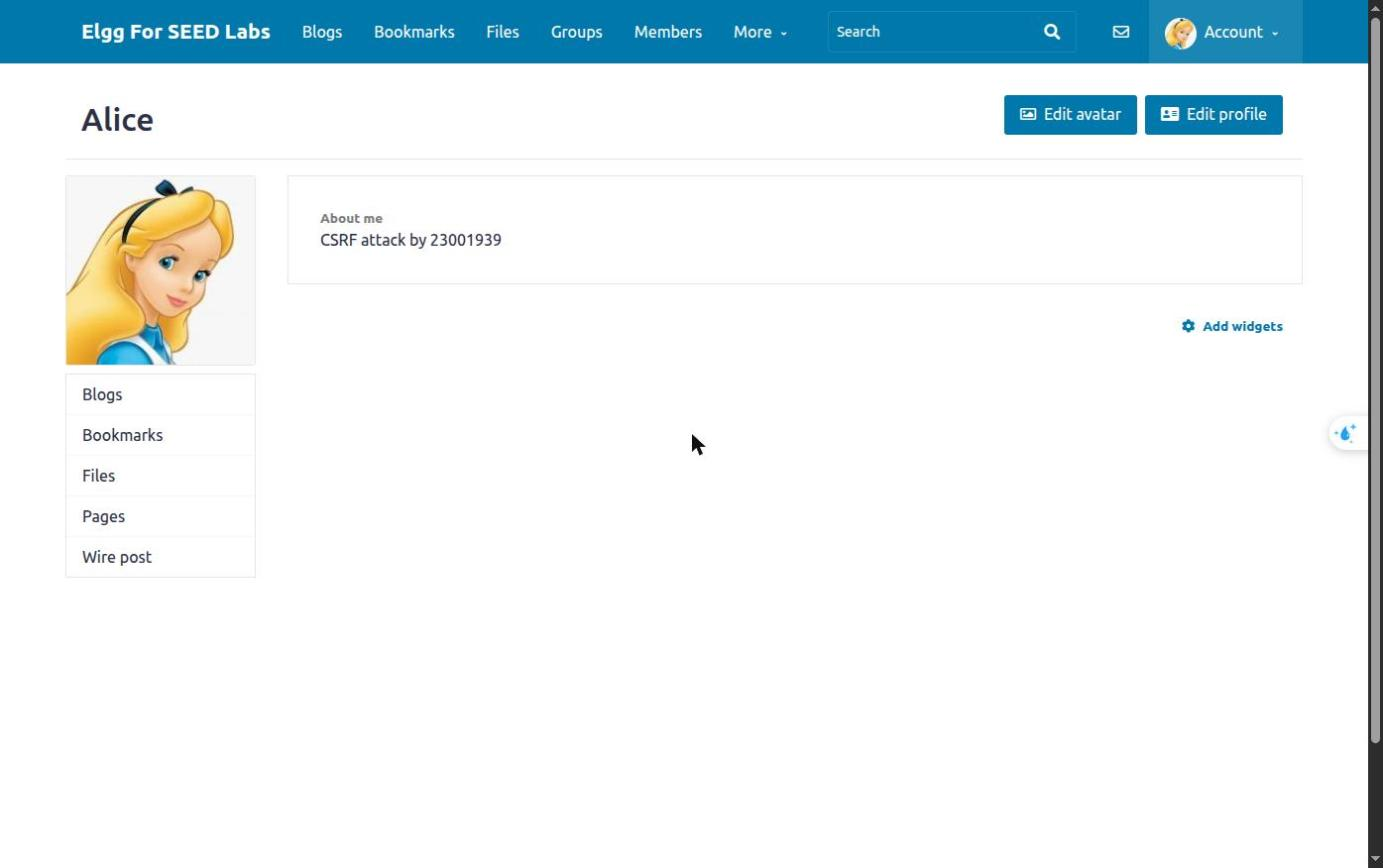
\includegraphics[width=\linewidth]{img/ev-after-success.jpg}}
  \\[3pt]\footnotesize\color{slate}(d) \textbf{TC-B06 (vulnerable, cùng-site):} About me = \texttt{CSRF attack by 23001939}.
\end{minipage}
\end{figure}

\begin{figure}[h]\centering
\begin{minipage}[t]{0.48\linewidth}\centering
  \fbox{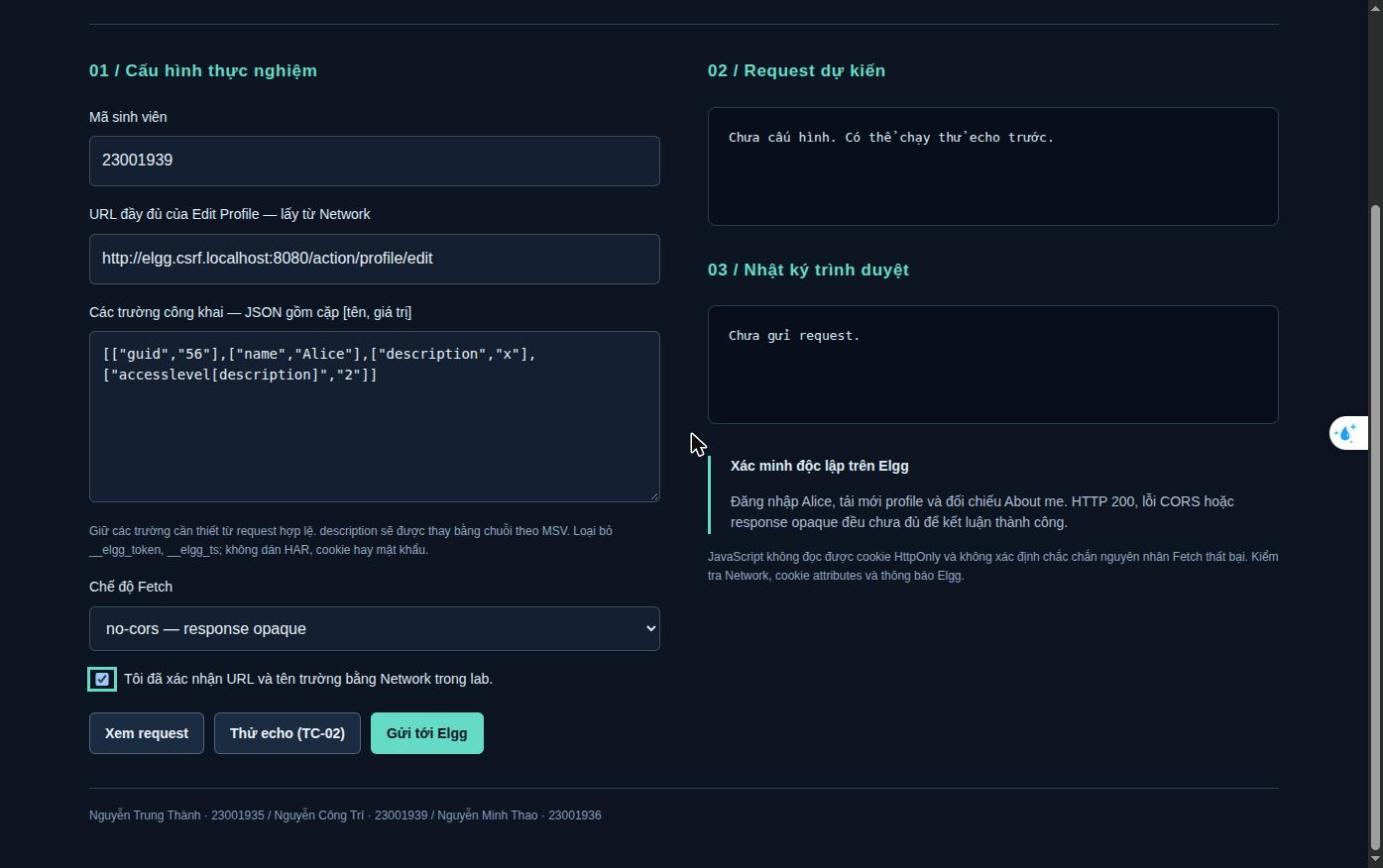
\includegraphics[width=\linewidth]{img/ev-attacker-config.jpg}}
  \\[3pt]\footnotesize\color{slate}(e) Giao diện attacker: cấu hình endpoint + các trường công khai (không token).
\end{minipage}\hfill
\begin{minipage}[t]{0.48\linewidth}\centering
  \fbox{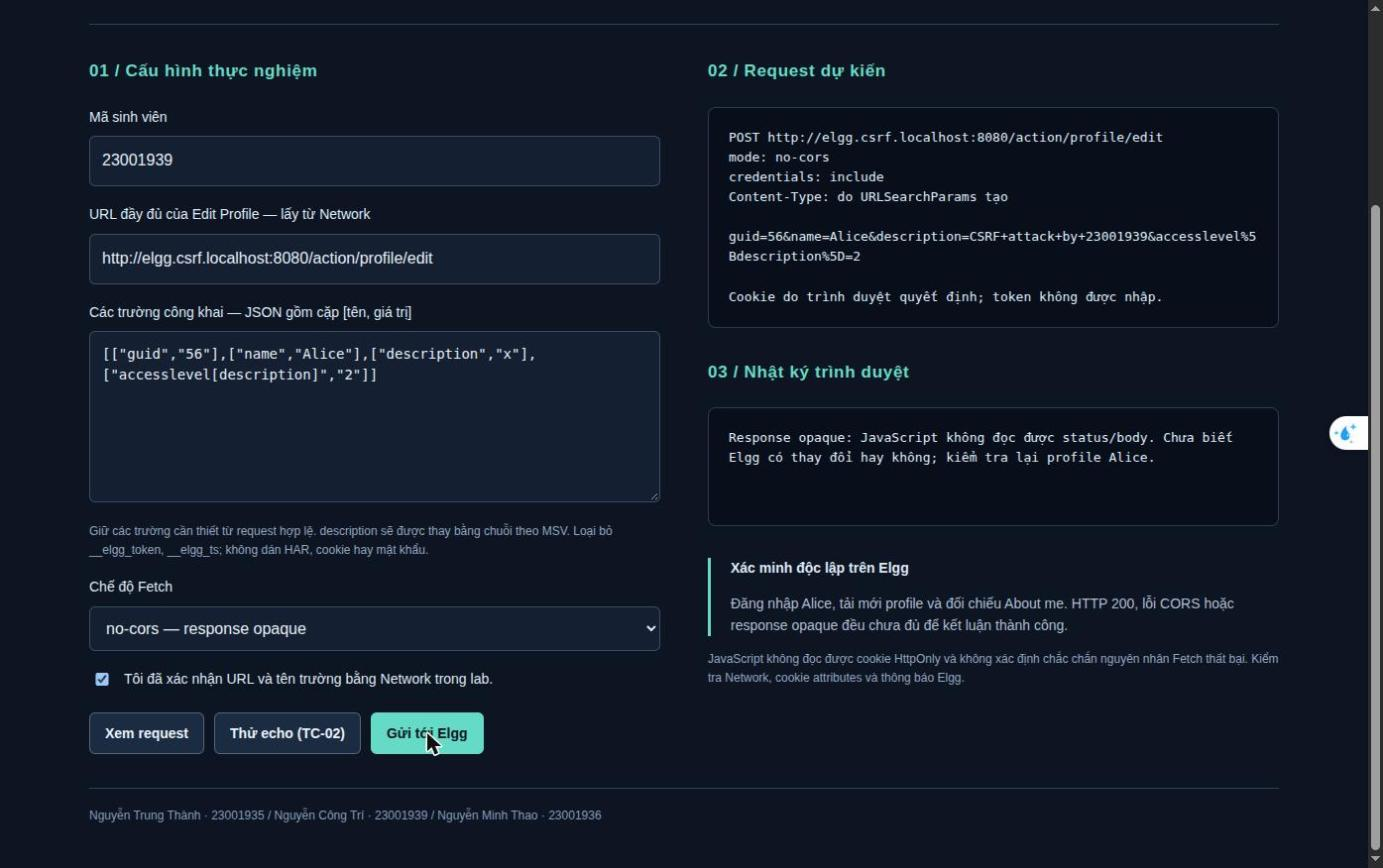
\includegraphics[width=\linewidth]{img/ev-crosssite.jpg}}
  \\[3pt]\footnotesize\color{slate}(f) \textbf{TC-B03:} tấn công từ \texttt{127.0.0.1} (khác-site) ở chế độ vulnerable — hồ sơ \emph{vẫn} không đổi.
\end{minipage}
\end{figure}

\begin{okbox}[Kết quả cốt lõi]
Ở chế độ \texttt{vulnerable} với attacker cùng-site, trường About me bị đổi thành \texttt{CSRF attack by 23001939} mà không có cảnh báo hay chuyển hướng — khai thác thành công hoàn toàn. Ngược lại, ở \texttt{protected} (token bật) cùng payload bị Elgg từ chối với thông báo thiếu token; và ở \texttt{vulnerable} nhưng khác-site, cookie SameSite khiến request mất phiên nên cũng không đổi được hồ sơ.
\end{okbox}

\subsection{Kiểm chứng ở tầng HTTP (curl)}
Để cô lập \emph{riêng} tác dụng của token (curl luôn tự đính cookie bất kể origin nên không xét SameSite), nhóm lặp lại POST \emph{thiếu token} bằng \texttt{curl}:
\begin{center}\small
\begin{tabularx}{\linewidth}{@{}l C C C@{}}
\toprule
\textbf{Chế độ} & \textbf{POST thiếu token} & \textbf{HTTP redirect} & \textbf{About me đổi?}\\
\midrule
protected & bị chặn & $\to$ \texttt{/} (home) & \no\\
vulnerable & chấp nhận & $\to$ \texttt{/profile/alice} & \yes\\
restored & — & — & \no\\
\bottomrule
\end{tabularx}
\end{center}
\noindent Sự khác biệt ở \emph{đích redirect} (home khi bị chặn, trang hồ sơ khi thành công) là một dấu hiệu phụ trợ rõ ràng, nhất quán với quan sát trên giao diện.

\subsection{Tường thuật chi tiết từng ca}
\begin{description}[leftmargin=1.6em,style=nextline]
  \item[TC-B01 — Đăng nhập \& Save hợp lệ.] Đăng nhập Alice, vào Edit Profile, đặt About me baseline, bấm Save. Request \texttt{POST /action/profile/edit} có đầy đủ \texttt{\_\_elgg\_token}/\texttt{\_\_elgg\_ts}; hồ sơ cập nhật đúng. Đây là mẫu để nhái và là đường khôi phục chuẩn.
  \item[TC-B04 — Protected chặn tấn công.] Giữ chế độ \texttt{protected}. Trang attacker cùng-site gửi POST (\texttt{credentials:'include'}, \texttt{no-cors}). Trình duyệt \emph{có} đính cookie (cùng-site) nhưng payload \emph{thiếu} token. Elgg hiển thị thông báo đỏ \emph{``Form is missing \_\_token or \_\_ts fields''}; About me giữ nguyên baseline.
  \item[TC-B03 — SameSite chặn khác-site.] Chuyển \texttt{vulnerable} (token tắt). Gửi từ \texttt{127.0.0.1} (khác-site). Cookie \texttt{SameSite} khiến trình duyệt \emph{không} đính phiên cho POST cross-site; Elgg coi là khách lạ nên không đổi hồ sơ — chứng minh SameSite bảo vệ \emph{độc lập} với token.
  \item[TC-B05/06 — Tấn công thành công.] Vẫn \texttt{vulnerable}, gửi từ attacker cùng-site. SameSite cho phép cookie cùng-site và token đã tắt $\Rightarrow$ Elgg chấp nhận. Tải lại hồ sơ: About me = \texttt{CSRF attack by 23001939}. Đây là bằng chứng hợp lệ duy nhất (đối chiếu trực tiếp trường hiển thị).
\end{description}

% =====================================================================
\section{Phát hiện kỹ thuật: annotation so với metadata}
Trong quá trình khôi phục hồ sơ, nhóm phát hiện một chi tiết triển khai quan trọng của Elgg:
\begin{itemize}
  \item Action web \texttt{/action/profile/edit} lưu trường About me dưới dạng \textbf{annotation} \texttt{profile:description} (bảng \texttt{elgg\_annotations}) — và đây chính là giá trị mà \emph{trang hồ sơ hiển thị}.
  \item Trong khi đó, thuộc tính PHP \texttt{\$user->description} ánh xạ sang \textbf{metadata} (bảng \texttt{elgg\_metadata}).
\end{itemize}
\textbf{Hệ quả:} công cụ \texttt{reset-profile} ban đầu chỉ đặt lại \emph{metadata}, nên tuy báo ``thành công'' nhưng trang vẫn hiển thị chuỗi tấn công; thao tác xoá cache (\texttt{elgg-cli flush}), khởi động lại container hay xoá Stash cache đều \emph{không} khắc phục vì dữ liệu nằm ở \emph{annotation}. Cách khôi phục đúng là sửa lại About me \emph{qua giao diện Edit Profile} (đi qua đúng action, ghi đè annotation), hoặc cập nhật trực tiếp annotation \texttt{profile:description}.

\begin{infobox}[Bài học]
Khi kiểm chứng kết quả, phải đối chiếu đúng \emph{nguồn dữ liệu mà giao diện hiển thị}. Một thay đổi ``thành công'' ở tầng DB nhưng sai bảng vẫn cho kết quả hiển thị sai. Phát hiện này cũng nhắc lại rằng lỗi CORS hay response opaque \emph{không} phải bằng chứng — chỉ việc đối chiếu trực tiếp trường hiển thị mới là bằng chứng hợp lệ.
\end{infobox}

% =====================================================================
\section{Kiểm chứng và phòng thủ}\label{sec:defense}
\subsection{Bật lại anti-CSRF token của Elgg}
Khi khôi phục cơ chế kiểm tra \texttt{\_\_elgg\_token}/\texttt{\_\_elgg\_ts}, chạy lại đúng payload cũ:
\begin{center}\small
\begin{tabularx}{\linewidth}{@{}Y C C@{}}
\toprule
 & \textbf{Phòng vệ TẮT} & \textbf{Phòng vệ BẬT}\\
\midrule
Payload có \texttt{\_\_elgg\_token}? & Không & Vẫn không\\
Phản hồi server & Cập nhật DB (302) & \textbf{Từ chối} (thiếu token)\\
About me của Alice & Bị đổi & \textbf{Không đổi}\\
\bottomrule
\end{tabularx}
\end{center}
\noindent Vì SOP cấm JavaScript của trang attacker đọc token nằm trên trang Elgg, request giả mạo luôn thiếu token hợp lệ $\Rightarrow$ bị chặn. Đây là bằng chứng trực quan cho \emph{Synchronizer Token Pattern}.

\subsection{Vai trò độc lập của cookie SameSite}
Thí nghiệm TC-B03 cho thấy: \emph{ngay cả khi} token đã tắt (\texttt{vulnerable}), một POST từ attacker \textbf{khác-site} (\texttt{127.0.0.1}) \emph{vẫn} không đổi được hồ sơ — vì trình duyệt không đính cookie phiên cho request cross-site (cookie \texttt{SameSite}). Elgg coi request là khách lạ nên không hành động thay Alice. Như vậy \textbf{mỗi lớp} (token hoặc SameSite), tự nó, đã đủ để chặn đòn tấn công này.

\subsection{Phòng thủ nhiều lớp (Defense-in-Depth)}
\begin{center}\small
\begin{tabularx}{\linewidth}{@{}l Y Y@{}}
\toprule
\textbf{Lớp} & \textbf{Biện pháp} & \textbf{Chặn được gì}\\
\midrule
Cookie & \texttt{SameSite=Lax/Strict} & Trình duyệt không gửi cookie cross-site\\
Ứng dụng & Anti-CSRF token (Synchronizer) & Attacker không đọc được token (nhờ SOP)\\
Ứng dụng & Double Submit Cookie & Attacker không đọc được cookie để nhét vào body\\
Header & Kiểm tra \texttt{Origin} / \texttt{Sec-Fetch-Site} & Từ chối request thay đổi trạng thái từ nguồn lạ\\
Giao diện & \texttt{X-Frame-Options} / CSP \texttt{frame-ancestors} & Chống Clickjacking qua iframe\\
\bottomrule
\end{tabularx}
\end{center}

\subsubsection{Giải thích cơ chế từng lớp}
\begin{itemize}
  \item \textbf{SameSite cookie:} do \emph{trình duyệt} thực thi. \texttt{Strict} chặn cookie cho mọi request khởi nguồn từ site khác; \texttt{Lax} (mặc định hiện nay) vẫn gửi cookie cho điều hướng cấp cao (gõ link, click) nhưng chặn cho POST ngầm cross-site — vừa đủ chặn CSRF mà không phá trải nghiệm. \emph{Hạn chế:} không bảo vệ tấn công \emph{same-site} (ví dụ subdomain bị chiếm).
  \item \textbf{Anti-CSRF token (Synchronizer):} do \emph{server} thực thi. Server nhúng token ngẫu nhiên theo phiên vào mỗi form; request hợp lệ phải trả đúng token. Nhờ SOP, attacker khác origin không đọc được token. \emph{Hạn chế:} cần quản lý vòng đời token; không chống XSS.
  \item \textbf{Double Submit Cookie:} server gửi token qua cả cookie và trường ẩn, rồi so khớp — không cần lưu trạng thái phía server. \emph{Hạn chế:} yếu nếu attacker ghi được cookie (ví dụ qua subdomain).
  \item \textbf{Kiểm tra \texttt{Origin}/\texttt{Sec-Fetch-Site}:} server từ chối request đổi trạng thái đến từ nguồn lạ. Đơn giản, hiệu quả cho API hiện đại. \emph{Hạn chế:} một số proxy/cấu hình có thể lược bỏ header.
\end{itemize}

\begin{infobox}[Khuyến nghị thực tế]
Kết hợp \texttt{SameSite=Lax} (lớp mặc định) + anti-CSRF token (lớp ứng dụng) + kiểm tra \texttt{Origin} cho endpoint nhạy cảm. Tuyệt đối không dùng \texttt{GET} cho hành động thay đổi trạng thái. Nguyên tắc \emph{phòng thủ nhiều lớp}: một lớp thất bại thì các lớp còn lại vẫn chặn được.
\end{infobox}

% =====================================================================
\section{Kiểm thử tự động và khả năng tái hiện}
Ngoài thực nghiệm thủ công, nhóm có bộ kiểm thử tự động để bảo đảm payload đúng chuẩn và môi trường lành mạnh:
\begin{center}\small
\begin{tabularx}{\linewidth}{@{}Y l c@{}}
\toprule
\textbf{Bộ test} & \textbf{Nội dung} & \textbf{Kết quả}\\
\midrule
\texttt{test\_request\_format.mjs} (Node) & 6 test dựng payload Fetch; chặn nhập token/cookie & \yes{} 6/6\\
\texttt{test\_environment.py} & 4 test attacker server: echo, allowlist tĩnh, không rò cookie & \yes{} 4/4\\
\texttt{test\_security\_controls.py} (live) & service healthy; Elgg không mở CORS & \yes{} 2/2\\
\texttt{docker compose config} & kiểm tra cú pháp compose & \yes\\
\bottomrule
\end{tabularx}
\end{center}

\begin{lstlisting}[language=bash,caption={Quy trình tái hiện lab (tóm tắt)}]
python3 lab/scripts/labctl.py up         # dung Elgg + MySQL + attacker
python3 lab/scripts/labctl.py version    # xac minh Elgg 3.3.3
# ... dang nhap Alice, bat request, cau hinh attacker, gui thu ...
python3 lab/scripts/labctl.py mode vulnerable   # tat token (co chu dich)
python3 lab/scripts/labctl.py mode protected    # bat lai token
python3 lab/scripts/labctl.py reset-profile     # khoi phuc About me
\end{lstlisting}

% =====================================================================
\section{Phân công công việc}
\begin{center}\small
\begin{tabularx}{\linewidth}{@{}l l Y@{}}
\toprule
\textbf{Thành viên} & \textbf{MSV} & \textbf{Trọng tâm}\\
\midrule
Nguyễn Trung Thành & 23001935 & Lý thuyết CSRF, phân tích HTTP request, phòng chống\\
Nguyễn Công Trí & 23001939 & Elgg, Docker, mã Fetch API, kiểm thử\\
Nguyễn Minh Thao & 23001936 & Bằng chứng, PowerPoint, video\\
\bottomrule
\end{tabularx}
\end{center}
\noindent \textbf{Nền tảng chung bắt buộc (100\% thành viên):} tự chạy Docker, tự bắt gói tin và tự đổi About me thành MSV của mình; cùng tham gia buổi vấn đáp chéo 15 câu hỏi.

% =====================================================================
\section{Khai báo mức độ sử dụng AI}
\begin{enumerate}
  \item \textbf{Mức 1 — Phản biện:} dùng AI thảo luận cơ chế \texttt{credentials: 'include'}, Simple Request và CORS; sinh viên tự viết mã.
  \item \textbf{Mức 2 — Đồng sáng tạo:} sinh viên thiết kế cấu trúc báo cáo/slide/sơ đồ, AI hỗ trợ trau chuốt câu từ và định dạng LaTeX.
  \item \textbf{Mức 3 — Tạo sinh theo prompt:} AI hỗ trợ sinh khung công cụ \texttt{labctl}/attacker và điều khiển automation kiểm thử; sinh viên cấu hình giá trị thật, chạy và chịu trách nhiệm kết quả.
\end{enumerate}
\noindent Mọi kết quả thực nghiệm và tính chính xác do nhóm trực tiếp chịu trách nhiệm.

% =====================================================================
\section{Thảo luận, hạn chế và hướng phát triển}
\subsection{Những điểm đã làm được}
\begin{itemize}
  \item Chạy thật end-to-end trên trình duyệt Chrome với Elgg 3.3.3; bằng chứng hình ảnh ở cả ba trạng thái (trước / bị chặn / thành công).
  \item Kiểm soát biến chặt chẽ để \emph{tách bạch} vai trò của anti-CSRF token và cookie SameSite.
  \item Tuân thủ nghiêm nguyên tắc đạo đức: không nhập token/cookie vào attacker; công cụ chủ động từ chối các trường bí mật.
\end{itemize}
\subsection{Hạn chế}
\begin{itemize}
  \item Mô hình SEED chuẩn (\texttt{www.seed-server.com}) chỉ trình bày ở mức khái niệm; mọi bằng chứng lấy từ lab Docker cục bộ của nhóm.
  \item Việc tắt token là \emph{chỉnh sửa có chủ đích} của lab để minh họa, không phải kết luận rằng bản Elgg hiện hành có lỗi.
  \item Response \texttt{no-cors} là opaque nên không đọc được mã trạng thái từ JS; kết luận chỉ dựa trên đối chiếu trực tiếp hồ sơ (đã xử lý đúng).
\end{itemize}
\subsection{Hướng phát triển}
\begin{itemize}
  \item Bổ sung kịch bản tấn công \emph{add friend} (chỉ cần guid của chính nạn nhân) để so sánh với kịch bản sửa profile.
  \item Thử nghiệm với các giá trị \texttt{SameSite} khác nhau (\texttt{Strict}/\texttt{Lax}/\texttt{None}) và quan sát trực tiếp việc đính/loại cookie trong tab Network.
  \item Sửa công cụ \texttt{reset-profile} để đặt lại đúng annotation \texttt{profile:description}.
\end{itemize}

% =====================================================================
\section{Kết luận}
Nhóm đã hoàn thành mục tiêu: đổi About me thành \texttt{CSRF attack by 23001939} bằng Fetch API (không dùng XHR/Form), phân tích đầy đủ cơ chế khai thác, \emph{chạy thật} trên lab Docker (Elgg 3.3.3) với bằng chứng hình ảnh, và \emph{chứng minh bằng thực nghiệm} hiệu quả của hai lớp phòng thủ độc lập (anti-CSRF token và cookie SameSite). Bài học cốt lõi: CSRF không bị HTTPS ngăn chặn; biện pháp căn cơ là \texttt{SameSite} cookie kết hợp anti-CSRF token và kiểm tra nguồn gốc request. Phát hiện về annotation/metadata cũng nhấn mạnh nguyên tắc: kết luận chỉ dựa trên bằng chứng đối chiếu trực tiếp, không dựa vào tín hiệu gián tiếp.

% =====================================================================
\appendix
\section{Phụ lục A: Lời giải 15 câu hỏi (tóm tắt)}
\small
\begin{enumerate}[leftmargin=2.2em]
\item \textbf{SameSite chống CSRF:} chỉ dẫn trình duyệt không gửi cookie trong request cross-site (Strict/Lax) $\Rightarrow$ request giả mạo mất phiên xác thực.
\item \textbf{Secret token:} server nhúng token ngẫu nhiên theo phiên vào form; nhờ SOP, attacker không đọc được token $\Rightarrow$ request giả thiếu token bị từ chối.
\item \textbf{HTTPS vẫn lo CSRF:} HTTPS chỉ bảo mật đường truyền; cookie vẫn được đính kèm trong đường hầm TLS, nên CSRF (lỗi tầng ứng dụng) không bị ngăn.
\item \textbf{GET \texttt{delete.php?pageid=5}:} dùng \texttt{<img src=...>} ẩn hoặc \texttt{fetch(...,\{credentials:'include'\})} để kích hoạt GET giả mạo.
\item \textbf{POST \texttt{delete.php}:} dùng Fetch + \texttt{URLSearchParams(pageid=5)}, chạy ngầm không chuyển trang.
\item \textbf{Tìm guid của Boby:} qua URL profile, \texttt{src} avatar, link Add friend, hoặc RSS feed — đều công khai.
\item \textbf{Không biết user id:} phụ thuộc server — nếu id suy ra từ session thì vẫn tấn công được; nếu bắt buộc id ngẫu nhiên lớn trong body thì không.
\item \textbf{Tấn công khách bất kỳ:} (1) \no{} sửa profile — cần guid nạn nhân mà SOP không cho đọc; (2) \yes{} add friend — chỉ cần guid của chính Alice, danh tính nạn nhân do session suy ra.
\item \textbf{Session ID trong data part (Double Submit):} cookie do trình duyệt tự gửi, nhưng data part phải do JS trang gốc gán; attacker không đọc được cookie nên không điền đúng $\Rightarrow$ server phát hiện cross-site.
\item \textbf{Trình duyệt biết cross-site?} Có — biết rõ origin nguồn và đích, gửi kèm \texttt{Origin}, \texttt{Sec-Fetch-Site}.
\item \textbf{Server biết cross-site?} Mặc định HTTP thuần thì không; biết được nếu kiểm tra \texttt{Origin}/\texttt{Referer}/\texttt{Sec-Fetch-Site}/token.
\item \textbf{Vì sao không chỉ dựa Referer:} Referer có thể bị bỏ hợp lệ (\texttt{Referrer-Policy}, HTTPS→HTTP, proxy) và dễ bị qua mặt bằng regex lỏng.
\item \textbf{Vì sao cần biết cross-site:} để chỉ cho phép hành động đổi trạng thái khi người dùng thực sự chủ ý, tránh bị mượn quyền.
\item \textbf{Cấm hẳn cookie cross-site?} Về kỹ thuật được nhưng phá vỡ điều hướng, SSO/OAuth, widget nhúng; giải pháp là \texttt{SameSite=Lax} mặc định.
\item \textbf{Iframe Facebook:} request từ trong iframe tới Facebook là same-site đối với Facebook (không cross-site); nguy cơ Clickjacking; bảo mật bằng \texttt{X-Frame-Options} / CSP \texttt{frame-ancestors}.
\end{enumerate}

\section{Phụ lục B: Thông tin tái hiện}
\small
\begin{itemize}
  \item \textbf{Phiên bản:} Elgg 3.3.3 (digest \texttt{sha256:5d8a25b1\ldots708f7f5}); MySQL 8.0.37; attacker Python 3.12.
  \item \textbf{Tài khoản SEED công khai (chỉ dùng trong lab):} Alice \texttt{alice}/\texttt{seedalice}; admin \texttt{admin}/\texttt{seedelgg}.
  \item \textbf{Chuỗi mục tiêu:} \texttt{CSRF attack by 23001939} (đổi theo MSV trong \texttt{.env} hoặc giao diện attacker).
  \item \textbf{Khôi phục:} \texttt{labctl mode protected} + sửa About me về baseline qua UI Edit Profile.
\end{itemize}

\begin{thebibliography}{9}\small
\bibitem{du} W. Du, \emph{Computer \& Internet Security: A Hands-on Approach}, 3rd ed.
\bibitem{fetch} WHATWG, \emph{Fetch Living Standard}, \url{https://fetch.spec.whatwg.org/}.
\bibitem{owasp} OWASP, \emph{Cross-Site Request Forgery Prevention Cheat Sheet}.
\bibitem{samesite} IETF, \emph{RFC 6265bis — Cookies: SameSite attribute}.
\bibitem{elgg} Elgg, \emph{Actions \& Security}, \url{https://learn.elgg.org/}.
\end{thebibliography}

\end{document}
